\documentclass{article}

\usepackage{icomp2026_conference}

\usepackage[T1]{fontenc}
\usepackage[utf8]{inputenc}
\usepackage{tempora}
\usepackage[english,russian]{babel}
\usepackage{hyperref}
\usepackage{url}
\usepackage{booktabs}
\usepackage{nicefrac}
\usepackage{microtype}
\usepackage{xcolor}
\usepackage{amsmath}
\usepackage{cleveref}
\usepackage{subcaption}
\usepackage{graphicx}
\usepackage{multirow}
\usepackage{amsmath,amssymb,amsfonts}
\usepackage{amsthm}
\usepackage{mathrsfs}
\usepackage{textcomp}
\usepackage{manyfoot}
\usepackage{algorithm}
\usepackage{algorithmicx}
\usepackage{algpseudocode}
\usepackage{listings}

\newtheorem{theorem}{Theorem}
\newtheorem{proposition}[theorem]{Proposition}
\newtheorem{lemma}{Lemma}
\newtheorem{example}{Example}
\newtheorem{remark}{Remark}
\newtheorem{definition}{Definition}
\newtheorem{assumption}{Assumption}
\newtheorem{hypothesis}{Hypothesis}    

\algrenewcommand{\algorithmicrequire}{\textbf{Input:}}
\algrenewcommand{\algorithmicensure}{\textbf{Output:}}


\title{SignMuon: fast as Muon, communication-efficient as SignSGD}

\author{
  Maria Smirnova\\
  MIPT\\
  Moscow, Russia\\
  \texttt{smirnova.ma@phystech.edu}\\
  \And
  Alexey Kravatskiy \\
  MIPT\\
  Moscow, Russia\\
  \texttt{kravatskii.aiu@phystech.edu}\\
}

\icompfinalcopy

\raggedbottom
\begin{document}

\maketitle

\begin{abstract}
Алгоритм знаковой компрессии градиентов SignSGD позволяет снизить объем передаваемых данных до 32 раз, что является критически важным для федеративного обучения в условиях ограниченной пропускной способности сети. Однако он зачастую уступает по качеству обучения современным оптимизаторам, таким как Muon, которые учитывают матричную структуру параметров. В данной работе представлен алгоритм SignMuon, который применяет знаковую компрессию к LMO-обновлению оптимизатора Muon. Эмпирические результаты экспериментов показывают, что SignMuon достигает точности, близкой к алгоритму Muon, и существенно превосходит SignSGD как в централизованном, так и в федеративном обучении.
    
\end{abstract}

\textbf{Keywords:} federated learning, stochastic optimization, gradient compression, 1-bit quantization, matrix orthogonalization, Linear Minimization Oracle (LMO), SignSGD, Muon.


\section{Введение}\label{sec:intro}
Современные методы обучения глубоких нейронных сетей требуют использования оптимизаторов, которые не только обеспечивают высокую скорость сходимости, но и минимизируют коммуникационные издержки в распределенных системах. В условиях федеративного обучения данные распределены между узлами, которые обмениваются информацией с сервером для обучения общей модели. Каждый узел имеет локальный набор данных, а целью федеративного обучения является минимизация усредненной функции потерь по всем узлам. В условиях низкой пропускной способности сети передача полных матриц обновлений модели может замедлять её скорость обучения. Для решения этой проблемы обычно используются методы компрессии градиентов \cite{bernstein2018signsgd,  bernstein2019signsgdmajority, beznosikov2020biased}. 

Так, алгоритм SignSGD продемонстрировал, что даже экстремальная компрессия (до 1 бита на компоненту) сохраняет работоспособность метода и позволяет сократить объём передаваемых данных примерно в 32 раза при незначительной потере качества модели по сравнению с SGD \cite{bernstein2018signsgd, bernstein2019signsgdmajority}. Однако SignSGD не учитывает матричную структуру параметров: в задачах с матричными весами он рассматривает матрицы как одномерные векторы (flattening), игнорируя их внутреннюю 2D-тензорную структуру, что может ухудшать качество обучения DNN. 

Недавно предложенный оптимизатор Muon показал, что его ортонормированные обновления стабилизируют обучение DNN и в ряде случаев превосходят стандартные адаптивные методы оптимизации по качеству итогового решения \cite{jordan2024muon, bernstein2024old, shah2025practical}. Оптимизатор Muon для матричных параметров реализует шаг steepest descent в спектральной норме. Согласно \citet{jordan2024muon}, Muon вычисляет направление обновления как ортонормированную матрицу $\mathbf{U}\mathbf{V}^\top$, где $\mathbf{U}$ и $\mathbf{V}$ -- ведущие сингулярные векторы градиента. Исходя из структуры алгоритма, Muon требует передачи полных матриц обновлений, что в федеративных задачах может быть слишком затратным.  

В данной работе мы предлагаем алгоритм SignMuon, который применяет знаковую компрессию к LMO-обновлению оптимизатора Muon. В отличие от SignSGD, который передаёт знак координат направления стохастического градиента, наш метод сначала вычисляет направление обновления с помощью LMO (Linear Minimization Oracle), как Muon, а затем передаёт только знак этого направления. Такая схема позволяет учитывать матричную структуру параметров и сохранять преимущества Muon, одновременно сокращая объём передаваемой информации до одного бита на координату. Тем самым SignMuon стремится объединить быструю сходимость структурированных оптимизаторов с коммуникационной эффективностью знаковых методов.

Эффективность предложенного оптимизатора показана на различных синтетических и прикладных задачах: 
% бенчмарк CIFAR-10 airbench \cite{jordan2023cifar10}, синтетический эксперимент по методу наименьших квадратов.
\begin{itemize}
    % \item Классификация изображений MNIST\cite{lecun2010mnist}
    \item Бенчмарк CIFAR-10 airbench \cite{jordan2023cifar10}
    \item Синтетический эксперимент по методу наименьших квадратов
    % \item Предварительное обучение (pre-training) моделей NanoGPT и GPT-2 Medium на датасете FineWeb \cite{jordan2024moddednanogpt}
\end{itemize}
Наши эксперименты направлены на изучение того, насколько эффективно можно сочетать структурированные направления обновления Muon с экстремальной коммуникационной компрессией знаковых методов. В частности, мы анализируем, как передача только знака направления обновления влияет на качество и устойчивость обучения по сравнению с использованием полного Muon-обновления.

Экспериментальные результаты показывают, что использование знаковой компрессии для направлений Muon позволяет снизить коммуникационные издержки (в 32 раза), сохраняя при этом темпы оптимизации. В централизованном сценарии алгоритм SignMuon превосходит базовый метод SignSGD по скорости сходимости и итоговой точности. При этом точность предложенного 1-битного метода уступает оптимизатору Muon всего на $1-1.5\%$, при этом уверенно превосходя базовые знаковые алгоритмы. В федеративном сценарии интеграция SignMuon с механизмами клиентского моментума и мажоритарного голосования (Majority Vote) обеспечивает стабильную сходимость и защиту от аномальных обновлений даже в условиях жесткого ограничения пропускной способности сети. Также, в работе представлен аналитический пример, который формализует границы применимости знаковой компрессии к LMO-обновлениям в детерминированном случае и решение гладкой выпуклой задачи. В результате проведенных экспериментов, предложенный подход демонстрирует, что LMO-основанные методы могут быть успешно объединены с знаковой компрессией без существенной потери качества обучения.

% Более того, предложенная схема естественным образом обобщается на более широкий класс алгоритмов SignA, где A обозначает любой оптимизатор, использующий LMO-направления. Это открывает возможность построения новых коммуникационно-эффективных алгоритмов оптимизации.


\section{Постановка задачи}\label{sec:proState}

\paragraph{Централизованное обучение} Рассмотрим стохастическую задачу оптимизации:
\begin{equation}
\min_{\mathbf{X} \in \mathcal{X}} \{f(\mathbf{X}) := \mathbb{E}_{\xi \sim \mathcal{D}} [f_{\xi}(\mathbf{X})]\},
\end{equation}
где $\mathcal{X}$ -- пространство параметров (например, $\mathbb{R}^d$ или $\mathbb{R}^{m \times n}$),  функции $f_{\xi} : \mathcal{X} \to \mathbb{R}$ могут быть невыпуклыми и негладкими, но являются непрерывно дифференцируемыми. Здесь $f_{\xi}(\mathbf{X})$ представляет собой функцию потерь модели с параметрами $\mathbf{X}$, вычисленную в точке обучающих данных $\xi$, выбранной из распределения вероятностей $\mathcal{D}$.

\paragraph{Федеративное обучение} В современном мире машинное обучение развивается благодаря масштабированию систем. Сегодняшние передовые модели опираются на массивные наборы данных и сложные архитектуры, требующие большого времени обучения. В современных реалиях задача обучения формулируется как поиск минимума в распределенной среде:


\begin{equation}
\min_{\mathbf{X} \in \mathcal{X}} \left\{ f(\mathbf{X}) := \frac{1}{N}\sum_{j=1}^N f_j(\mathbf{X})\right\}, \quad f_j(\mathbf{X})=\mathbb{E}_{\xi_j\sim \mathcal{D}_j}[f(\mathbf{X},\xi_j)]
\label{fed_eq}
\end{equation}
где $\mathcal{X}$ -- пространство параметров (например, $\mathbb{R}^d$ или $\mathbb{R}^{m \times n}$), $\mathbf{X} \in \mathcal{X}$ -- параметры модели, $N \ge 1$ -- количество узлов/клиентов/машин, а $f_j(\mathbf{X})$ -- функция потерь модели $\mathbf{X}$ на данных ($\mathcal{D}_j$), хранящихся на узле $j \in [N] := \{1, \dots, N\}$. В федеративном режиме узлы вычисляют локальные стохастические градиенты и периодически отправляют сообщения на сервер, канал коммуникации часто ограничен, поэтому критическим ресурсом является объём передаваемых данных \cite{bernstein2019signsgdmajority, horvath2023stochastic}. Некоторые практические приёмы в федеративном обучении и компрессии также рассмотрены в \cite{beznosikov2020biased, gruntkowska2025error, ahn2025dion}.

Для теоретического анализа оптимизации в таких распределенных условиях мы опираемся на предположение об $L$-гладкости функции $f$ в неевклидовом пространстве, оснащенном нормой $\|\cdot\|$. Формально это означает, что для любых $\mathbf{X}, \mathbf{Y} \in \mathbb{R}^d$ выполняется:
\begin{equation}
\|\nabla f(\mathbf{X}) - \nabla f(\mathbf{Y})\|_* \leq L \|\mathbf{X} - \mathbf{Y}\|,
\end{equation}
где $\|\cdot\|_*$ -- дуальная норма, определяемая как $\|\mathbf{X}\|_* := \sup_{\|\mathbf{X}'\| \leq 1} \langle \mathbf{X}, \mathbf{X}' \rangle \text{ для всех } \mathbf{X} \in \mathbb{R}^d$ \cite{kovalev2025understanding}. Отметим, что на практике также возможно использование ослабленных условий гладкости типа $(L_0,L_1)$ \cite{pethick2025generalized}. В свою очередь, жесткие ограничения на пропускную способность сети делают передачу полных 32-битных градиентов неэффективной. Исходя из этого, в данной работе целесообразно рассмотреть сценарии с экстремальной компрессией, где целевой уровень сжатия составляет 1 бит на компоненту сообщения \cite{bernstein2018signsgd, bernstein2019signsgdmajority, beznosikov2020biased}.

\textbf{Linear Minimization Oracle (LMO)} -- оператор $A(\cdot)$ как решение задачи линейной минимизации на допустимом множестве:
\begin{equation}
A(\mathbf{X})=\arg\min_{\mathbf{Y} \in \mathcal{S}}\langle \mathbf{X}, \mathbf{Y}\rangle.
\end{equation}
где $\mathbf{X}\in\mathbb{R}^{m\times n}$ -- эффективное направление обновления, $\mathcal{S}\subset\mathbb{R}^{m\times n}$ -- множество ограничений (convex set) и $\langle \mathbf{X},\mathbf{Y}\rangle=\sum_{i,j}{X}_{ij}{Y}_{ij}$ -- стандартное скалярное произведение матриц \cite{pethick2025training}. В частности, ограничения можно задать через единичный шар некоторой нормы:
\begin{equation}
A(\mathbf{X})=\arg\min_{\mathbf{Y} \in \{ \mathbf{Y} \in \mathcal{S} | \|\mathbf{Y}\| \le1\}}\langle \mathbf{X}, \mathbf{Y}\rangle.
\end{equation}
Такой оператор выбирает направление наискорейшего спуска в заданной норме. Аналитическая и практическая роль LMO подробно обсуждается в работах по норм-ограниченным LMO-оптимизаторам \cite{pethick2025training, kovalev2025understanding, riabinin2025gluon}.

\textbf{Оптимизатор Muon} использует матричную структуру градиента. Muon реализует шаг steepest descent в спектральной норме, где направление обновления получается ортогонализацией матрицы градиента \cite{bernstein2024old}. Пусть $\mathbf{M}=\mathbf{U}\boldsymbol{\Sigma}\mathbf{V}^\top$ -- сингулярное разложение матрицы $\mathbf{M}\in\mathbb{R}^{m\times n}$, где $\mathbf{U}\in\mathbb{R}^{m\times r}$, $\mathbf{V}\in\mathbb{R}^{n\times r}$ -- ортонормированные матрицы сингулярных векторов, $\boldsymbol{\Sigma}\in\mathbb{R}^{r\times r}$ -- диагональная матрица сингулярных значений, $r=\mathrm{rank}(\mathbf{M})$. Тогда LMO-направление имеет вид:
\begin{equation}
A(\mathbf{M})=\mathbf{U}\mathbf{V}^\top \in \mathbb{R}^{m\times n}.
\end{equation}
то есть выбирается ортонормированное направление, соответствующее решению задачи линейной минимизации. На практике Muon использует сглаженную оценку градиента с моментумом и его обновление выглядит следующим образом: 
\begin{equation}
    \begin{aligned}
        \mathbf{M}_t &= \mu \mathbf{M}_{t-1} + \mathbf{G}_t, \\
        \mathbf{M}_t &= \mathbf{U}_t \boldsymbol{\Sigma}_t \mathbf{V}_t^\top, \\
        \mathbf{D}_t &= \mathbf{U}_t \mathbf{V}_t^\top, \\
        \mathbf{X}_{t+1} &= \mathbf{X}_t - \eta_t \mathbf{D}_t.
    \end{aligned}
\end{equation}

В исходной реализации Muon вычисление $\mathbf{U}_t\mathbf{V}_t^\top$ выполняется приближённо с помощью итераций Ньютона-Шульца и других полиномиальных схем, что позволяет эффективно ортогонализовать матрицу без явного вычисления SVD \cite{amsel2025polar, li2025note, liu2025muon}. Интуитивно такая ортогонализация делает обновления изотропными и предотвращает доминирование нескольких направлений градиента, что особенно важно при обучении DNN \cite{bernstein2024old, shah2025practical}.

% \textbf{Класс алгоритмов SignA и SignMuon}
% \\Обозначим знаковую компрессию через поэлементную функцию $\operatorname{sign}(\cdot)$, которая переводит каждый элемент матрицы (или вектора) в $\pm 1$. Определим класс алгоритмов SignA как:
% \begin{equation}
% \begin{aligned}
% A(\mathbf{G}_t) &\colon \mathbf{G}_t \mapsto \mathbf{D}_t, \\
% \mathbf{s}_t &= \operatorname{sign}(\mathbf{D}_t) \in \{\pm 1\}^{m \times n}, \\
% \mathbf{X}_{t+1} &= \mathbf{X}_t - \eta_t \hat{\mathbf{s}}_t,
% \end{aligned}
% \end{equation}
% где $\mathbf{G}_t, \mathbf{D}_t, \mathbf{X}_t \in \mathbb{R}^{m \times n}$, $\hat{\mathbf{s}}_t$ -- агрегированное сообщение (в централизованном случае $\hat{\mathbf{s}}_t = \mathbf{s}_t$, в федеративном -- majority-vote или усреднение по узлам). Частным случаем данного семейства алгоритмов является SignMuon, где оператор $A$ соответствует Muon (т.е. $\mathbf{D}_t=\mathbf{U}_t\mathbf{V}_t^\top$), и передаётся только $\operatorname{sign}(\mathbf{U}_t\mathbf{V}_t^\top)$ \cite{petrov2025leveraging}.

% SignA реализует шаг steepest-descent с ограничением по норме и LMO-направлением:
% \begin{equation}
% \mathbf{X}_{t+1} = \mathbf{X}_t - \eta_t \operatorname{sign}\Big(\arg\min_{\|\mathbf{D}\|\le 1}\langle \mathbf{G}_t, \mathbf{D}\rangle\Big).
% \end{equation}

Несмотря на теоретические и практические преимущества, алгоритм Muon требует передачи полной ортогонализованной матрицы $\mathbf{D}_t$, что делает его крайне затратным в применении в федеративном обучении. Наша цель -- сконструировать коммуникационно-эффективный метод, который сохраняет геометрические свойства LMO-обновления Muon, но снижает нагрузку на сеть до уровня алгоритма SignSGD (1 бит на параметр), обеспечивая при этом стандартные теоретические гарантии сходимости в невыпуклом случае:
\begin{equation}
\min_{0 \le t \le T}\mathbb{E}\bigl[\|\nabla f(\mathbf{X}_t)\|_*^2\bigr] = \mathcal{O}(T^{-1/2}).
\end{equation}


\section{Теория}\label{sec:theory}
Рассмотрим семейство алгоритмов SignA, где A обозначает любой оптимизатор, использующий LMO-направления. Все алгоритмы семейства построены по единой структуре, состоящей из трёх последовательных этапов: обработка моментума, вычисление LMO-направления и знаковая компрессия обновления. 

В формальной постановке класс алгоритмов SignA инициализирует буфер моментума $\mathbf{M}_0 = \mathbf{0}$, а затем на каждой итерации $t \ge 1$ выполняет следующую последовательность обновлений:
\begin{equation}
\begin{aligned}
\mathbf{M}_t &= \mu \mathbf{M}_{t-1} + \mathbf{G}_t && \text{(Momentum accumulation)}\\
\tilde{\mathbf{M}}_t &= 
\begin{cases} 
    \mathbf{G}_t + \mu \mathbf{M}_t & \text{(Nesterov momentum)}, \\
    \mathbf{M}_t & \text{(otherwise)}
\end{cases} && \text{(Effective direction)}, \\
\mathbf{D}_t &= A(\tilde{\mathbf{M}}_t), && \text{(LMO projection)} \\
\mathbf{s}_t &= \operatorname{sign}(\mathbf{D}_t) \in \{\pm 1\}^{m \times n},  && \text{(Sign compression)}\\
\mathbf{X}_{t+1} &= \mathbf{X}_t - \eta_t \lambda_{\mathrm{mult}} \mathbf{s}_t && \text{(Parameter update)},
\end{aligned}
\label{eq:signa_general}
\end{equation}
 где $\mathbf{X}_t \in \mathbb{R}^{m \times n}$ -- текущая матрица параметров модели, $\mathbf{G}_t$ -- её стохастический градиент, $\mu \in [0, 1)$ -- коэффициент моментума, $\eta_t$ -- темп обучения (learning rate), а $\lambda_{\mathrm{mult}} > 0$ -- опциональный масштабирующий множитель (по умолчанию $\lambda_{\mathrm{mult}}=1$). Оператор $A(\cdot)$ обозначает LMO-оракул в заданной неевклидовой норме, а функция $\operatorname{sign}(\cdot)$ применяется поэлементно к полученному структурному направлению $\mathbf{D}_t$.

Предлагаемый в работе метод SignMuon является частным случаем класса алгоритмов SignA, он объединяет ортогонализованные LMO-направления оптимизатора Muon с экстремальной знаковой компрессией SignSGD. Ниже описаны две основные реализации данного алгоритма -- централизованная и федеративная.

\subsection{Централизованный сценарий}
В централизованной постановке алгоритм SignMuon применяется к матричным параметрам модели. Практическая реализация алгоритма учитывает тензорную структуру параметров нейронной сети. Процесс оптимизации разделен на два потока: матричные параметры (веса сверточных и полносвязных слоев, $n_{dim} \ge 2$) обновляются с помощью LMO-алгоритма SignMuon, а векторные параметры (bias, Batch Normalization layer, $n_{dim} = 1$) и последний слой классификатора оптимизируются стандартным методом AdamW. Первоначально такой подход был предложен в эмпирическом описании \cite{jordan2024muon}. Первый результат о теоретической сходимости был получен Li и Hong, которые проанализировали гладкую невыпуклую постановку \cite{li2025note}, а также формализован в рамках фреймворка Gluon \cite{riabinin2025gluon}.

Для матричных параметров ключевым этапом алгоритма SignMuon является поиск ортонормированного LMO-направления $\mathbf{D}_t \approx \mathbf{U}_t \mathbf{V}_t^\top$. Чтобы избежать высоких вычислительных затрат на явное вычисление сингулярного разложения (SVD) на каждом шаге оптимизации, на практике применяется итерационный алгоритм Ньютона-Шульца 5-го порядка. В ортогонализации Ньютона-Шульца мы приняли коэффициенты равными $a=3.4445, b=4.7750, c=2.0315$. Отличие нашего подхода от классического SignSGD заключается в том, к какому объекту применяется компрессия. Если в SignSGD знаковая компрессия применяется непосредственно к стохастическому градиенту, то в SignMuon сначала строится структурированное направление обновления $\mathbf{D}_t$, соответствующее LMO-шагу Muon, и лишь затем полученная матрица сжимается поэлементной функцией $\operatorname{sign}(\mathbf{D}_t)$. Тем самым SignMuon сохраняет геометрию ортонормированных обновлений и одновременно снижает объём передаваемой информации до одного бита на компоненту. Полная логика обновления матричных параметров представлена в Приложении ~\ref{app:central_alg}.

\subsection{Федеративный сценарий}
В федеративном обучении данные распределены между $N$ узлами. Каждый узел $j$ имеет свой локальный набор данных $\mathcal{D}_j$ и вычисляет локальную функцию потерь $f_j(\mathbf{X})$. Цель обучения состоит в минимизации усреднённой по всем узлам функции потерь (\ref{fed_eq}). Узлы не обмениваются данными между собой, они передают на сервер сжатые сообщения, что делает коммуникацию в федеративном обучении узким местом.

В федеративном сценарии использования алгоритма SignMuon сервер выполняет роль агрегатора, а основная структурная оптимизация происходит на узлах. В начале раунда $t$ каждый узел $j$ копирует глобальную модель. Вместо выполнения локальных шагов изменения параметров, узел вычисляет усреднённый стохастический градиент, накапливая его по $\mathrm{n\_steps}$ мини-батчам локальных данных. Этот приём (Gradient Accumulation) снижает дисперсию оценки перед применением LMO-оракула. Формально, накопленный градиент равен:
$$
\mathbf{G}_t^{(j)}\gets\frac{1}{n_{\text{steps}}}\sum_{i=1}^{n_{\text{steps}}}\nabla f(\mathbf{X}_t;\xi_{t,i}^{(j)}).
$$
В соответствии с общей логикой семейства SignA (\ref{eq:signa_general}), каждый узел поддерживает свой локальный буфер моментума $\mathbf{M}_t^{(j)}$. Узел обновляет моментум, применяет к нему LMO-оракул (Newton-Schulz) и выполняет знаковую компрессию:
$$ \mathbf{M}_t^{(j)} = \mu \mathbf{M}_{t-1}^{(j)} + \mathbf{G}_t^{(j)} $$
$$ \mathbf{s}_t^{(j)} = \operatorname{sign}\bigl(A(\mathbf{M}_t^{(j)})\bigr) \in \{\pm 1\}^{m \times n} $$
где $t\in[0, \mathrm{rounds}-1]$, $A(\cdot)$ -- оператор Muon (Newton-Schulz ортогонализация с параметрами $a=3.4445, b=4.7750, c=2.0315$). Таким образом, каждый узел передаёт на сервер лишь 1 бит на компонент матричного параметра.

На сервере поступившие от узла сообщения агрегируются с помощью majority-vote. Обозначим агрегированный знак через $\mathbf{s}_t^{\mathrm{agg}}$, тогда он задаётся формулой:
\begin{equation}
\mathbf{s}_t^{\mathrm{agg}}=\operatorname{sign}\!\left(\sum_{j=1}^N \mathbf{s}_t^{(j)}\right).
\end{equation}
Операция majority-vote гарантирует, что результирующий знак $\mathbf{s}_t^{\mathrm{agg}}$ равен $+1$ или $-1$ в каждой компоненте и соответствует «мнению большинства» узлов. Поскольку моментум уже был учтен на стороне узлов, сервер напрямую обновляет глобальную модель матричных параметров:
\[
\mathbf{X}_{t+1} = \mathbf{X}_t - \eta_t \mathbf{s}_t^{\mathrm{agg}}.
\]
Отдельно следует отметить обработку последних (классификационных) слоёв  модели. Эти параметры не обновляются SignMuon-правилом, а оптимизируются с помощью AdamW. Полная логика федеративного алгоритма SignMuon представлена в Приложении ~\ref{app:fed_alg}.

\subsection{Федеративный сценарий -- Error Feedback algorithm}
Алгоритм Federated SignMuon демонстрирует эмпирическую стабильность, однако знаковая компрессия неизбежно вносит смещение (bias) в направление спуска. Чтобы компенсировать ошибку квантования и обеспечить строгие гарантии сходимости, мы интегрируем в наш метод механизм Error Feedback, адаптированный для LMO-оптимизаторов в недавней работе Gruntkowska et al. \cite{gruntkowska2025error}. 

В данной модификации Federated EF-SignMuon процедура ортогонализации (LMO) переносится на сервер. Узлы не вычисляют LMO локально, вместо этого они вычисляют разность между текущим локальным моментумом и предыдущей оценкой градиента, после чего применяют к ней знаковую компрессию. Сервер агрегирует эти сжатые обновления, восстанавливает глобальную оценку градиента и только затем применяет к ней оператор Muon. Полный алгоритм представлен в Приложении ~\ref{app:ef21_alg}. Передача дополнительного скаляра $\alpha_t^{(j)}$ для каждого слоя практически не увеличивает размер сообщения, сохраняя общий объем трафика на уровне $\approx 1$ бита на параметр. Таким образом, обе предложенные архитектуры федеративного SignMuon: как базовая схема с мажоритарным голосованием, так и модификация с компенсацией ошибки -- успешно решают проблему коммуникационного узкого места. Они позволяют сохранить геометрические преимущества матричной ортогонализации Muon, обеспечивая при этом экстремально низкую нагрузку на сеть.

\subsection{Теоретические ограничения}
Предложенные гипотезы ~\ref{app:hyp} опираются на предположение о том, что направление наискорейшего спуска в спектральной норме (LMO-шаг алгоритма Muon) остается направлением убывания и после применения экстремальной знаковой компрессии. Однако это не всегда верно. 

В классическом алгоритме градиентного спуска гарантируется, что направление антиградиента $(-\mathbf{G}_t)$ всегда обеспечивает убывание функции, так как скалярное произведение градиента с самим собой строго положительно: $\langle \mathbf{G}_t, \mathbf{G}_t \rangle > 0$. В алгоритме SignMuon направление шага задается матрицей $\mathbf{s}_t = \operatorname{sign}(\mathbf{U}_t \mathbf{V}_t^\top)$. Чтобы алгоритм гарантированно сходился, необходимо выполнение условия убывания (Descent Condition):
\begin{equation}
\langle \mathbf{G}_t, \operatorname{sign}(\mathbf{U}_t \mathbf{V}_t^\top) \rangle > 0.
\label{eq:descent_condition}
\end{equation}
Возникает вопрос: гарантирует ли спектральная ортогонализация выполнение неравенства (\ref{eq:descent_condition}) для любых матриц? Данный вопрос формализуется следующей теоремой. 

\begin{theorem}\label{th:1} Существуют такие функции $f(W)$ и размерности $N \geq 4$, для которых алгоритм SignMuon строго расходится.
\end{theorem}

В качестве доказательства приведен пример в приложении~\ref{app:proof_th1}. Cуществование примера показывает, что алгоритм SignMuon не имеет глобальных гарантий сходимости для произвольных функций. Для обоснования его успешной работы на реальных задачах глубокого обучения (где алгоритм демонстрирует высокую точность) необходимо введение дополнительных предположений.

\section{Эксперименты}
Целью данных экспериментов является эмпирическая валидация алгоритма SignMuon, как оптимизатора, объединяющего высокую скорость сходимости LMO-оптимизаторов с коммуникационной эффективностью знаковой компрессии. Само исследование состоит из нескольких частей, включая валидацию в централизованном и федеративном случае, а также проверку алгоритма на синтетическом эксперименте по методу наименьших квадратов.

\subsection{Гладкая выпуклая задача (Синтетический тест)}
Для того чтобы оценить влияние матричной структуры на ход оптимизации (без влияния стохастического шума и сложной архитектуры нейронных сетей), мы начинаем эксперименты с детерминированной $L-$гладкой выпуклой задачи. Для этого рассмотрим задачу минимизации квадратичной формы:
\begin{equation}
F(\mathbf{X}) = \frac{1}{2} \|\mathbf{M}^{1/2} \mathbf{X} \mathbf{N}^{1/2}\|_F^2 = \frac{1}{2} \langle \mathbf{X}, \mathbf{M} \mathbf{X} \mathbf{N} \rangle \to \min_{\mathbf{X} \in \mathbb{R}^{m \times n}},
\label{eq:synthetic_problem}
\end{equation}
где матрица параметров $\mathbf{X} \in \mathbb{R}^{m \times n}$ имеет размерность $m = n = 500$, что соответствует типичным размерам матрицы весов DNN. Матрицы $\mathbf{M} \in \mathbb{S}_+^m$ и $\mathbf{N} \in \mathbb{S}_+^n$ являются симметричными положительно полуопределёнными. Для генерации данных мы случайным образом задаем спектры матриц $\mathbf{M}$ и $\mathbf{N}$, равномерно распределяя их собственные значения на интервале $(0, 1)$, что гарантирует константу гладкости $L \le 1$ относительно нормы Фробениуса. Начальное приближение матрицы $\mathbf{X}_0$ инициализируется элементами, сэмплированными независимо из нормального распределения $\mathcal{N}(0, 0.01)$.

Поскольку теоретические оценки скорости сходимости зависят от выбора нормы и констант гладкости, будем использовать эмпирический критерий эффективности: алгоритмы оцениваются по минимальному количеству итераций, необходимых для достижения порогового значения функции потерь $F(\mathbf{X}) \le 0.001$, максимальное число итераций $T_{\max} = 5000$. Для поиска оптимальных гиперпараметров оптимизаторов был проведен сеточный поиск (Grid Search) по learning rate $\eta$ и коэффициенту моментума $\mu$ для каждого из пяти рассматриваемых оптимизаторов (SignMuon, Muon, SignSGD, SGD и Adam):
\begin{itemize}
    \item $\mu \in \{0.1, 0.2, 0.3, 0.4, 0.5, 0.6, 0.7, 0.8, 0.9, 0.95\}$ для всех алгоритмов, кроме Adam;
    \item $\eta \in [0.005, 0.020]$ с шагом $0.001$ для Muon;
    \item $\eta \in [1\cdot 10^{-4}, 0.001]$ с шагом $10^{-4}$ для SignMuon;
    \item $\eta \in [5\cdot 10^{-5}, 2\cdot 10^{-4}]$ с шагом $10^{-5}$ для SignSGD;
    \item $\eta \in [0.01, 0.10]$ с шагом $0.01$ для SGD и Adam.
\end{itemize}

Результаты сеточного поиска и итоговое количество итераций до достижения необходимой точности в 0.001 представлены в Таблице \ref{tab:synthetic_results}. Из результатов видно, что алгоритм Muon достиг оптимума за 1122 итерации, что сопоставимо с классическими методами первого порядка (Adam, SGD). Стоит отметить, что алгоритм SignMuon достигает целевого значения функции потерь за 2104 итерации, значительно превосходя базовый алгоритм SignSGD (3120 итераций). Динамика целевой функции и нормы градиента в процессе оптимизации проиллюстрированы в Приложении на Рисунке \ref{fig:synthetic_results}.

\begin{table}[H]
\centering
\caption{Сравнение оптимизаторов на гладкой выпуклой задаче (уравнение \ref{eq:synthetic_problem}). Показаны оптимальные гиперпараметры, обеспечивающие достижение $F(\mathbf{X}) \le 0.001$ за наименьшее число итераций.}
\label{tab:synthetic_results}
\small
\renewcommand{\arraystretch}{1.2}
\begin{tabular}{|l|c|c|c|}
\hline
Algorithm & learning rate ($\eta$) & momentum ($\mu$) & Iterations to $0.001$ \\
\hline
SignMuon & 0.0002 & 0.2 & 2104 \\
Muon & 0.0065 & 0.1 & 1122 \\
SignSGD & 0.00015 & 0.8 & 3120 \\
SGD & 0.1 & 0.95 & 972 \\
Adam &  0.07 & - & 202 \\
\hline
\end{tabular}
\end{table}



\subsection{Централизованное обучение}
В данном эксперименте мы сравниваем динамики сходимости и итоговые точности (Accuracy) алгоритма SignMuon с классическими оптимизаторами Muon, SignSGD, SGD и Adam при фиксированном количестве эпох. Одной из задач эксперимента является демонстрация того, что SignMuon обеспечивает высокое качество классификации, сопоставимое с Muon, при этом превосходит по точности классический алгоритм SignSGD при идентичной коммуникации (1 бит на параметр).  

% Эксперименты проводились на датасетах MNIST и CIFAR-10:
% \begin{itemize}
%     \item \textbf{CIFAR-10:} Стандартный датасет для задачи классификации изображений. Содержит 60 000 цветных изображений 10 классов. Каждое изображение представлено в виде тензора размерности $3 \times 32 \times 32$, где первый индекс соответствует количеству цветовых каналов (RGB). Для централизованного обучения датасет делится на обучающую и тестовую выборки. В федеративном сценарии обучающая выборка делится между узлами.
%     \item \textbf{MNIST:} Датасет для задачи классификации изображений, используемый в бенчмарках распределенного обучения. Содержит 70 000 черно-белых изображений рукописных цифр (10 классов, по классу на каждую цифру) размером $28 \times 28$ пикселей (1 канал). Как и в случае с CIFAR-10, для централизованного обучения датасет делится на обучающую и тестовую выборки, а для федеративного сценария обучающая выборка делится между узлами.
% \end{itemize}

Эксперименты проводились на датасете CIFAR-10: стандартный датасет для задачи классификации изображений. Содержит 60 000 цветных изображений 10 классов. Каждое изображение представлено в виде тензора размерности $3 \times 32 \times 32$, где первый индекс соответствует количеству цветовых каналов (RGB). Для централизованного обучения датасет делится на обучающую и тестовую выборки. В федеративном сценарии обучающая выборка делится между узлами.

В качестве базовой модели была использована архитектура ResNet-18, адаптированная под изображения малого разрешения за счет использования начальной свертки $3\times3$ без макс-пулинга. Сеть включает четыре блока остаточных слоев (Residual Blocks) с пакетной нормализацией (BatchNorm), завершаясь слоем регуляризации Dropout и линейным классификатором. Как было сказано ранее обучение происходило при фиксированном количестве эпох $T_{max}=75$. В процессе обучения learning rate варьируется, используя косинусный планировщик скорости обучения (CosineAnnealingLR). Обновление learning rate $\eta_t$ на эпохе $t$ осуществляется по следующей формуле:
\begin{equation}
\eta_t = \eta_{\text{min}} + \frac{1}{2}(\eta_{\text{max}} - \eta_{\text{min}})\left(1 + \cos\left(\frac{t}{T_{\text{max}}}\pi\right)\right),
\end{equation}
где $\eta_{\text{max}}$ -- начальный learning rate алгоритма, $\eta_{\text{min}} = 0$ -- минимальное значение (в нашей конфигурации), а $T_{\text{max}}$ соответствует общему числу эпох обучения. 

Результаты эксперимента и значения подобранных гиперпараметров указаны в Таблице \ref{tab:cifar_central}. Динамика целевой функции и точности алгоритмов в процессе обучения проиллюстрированы в Приложении~\ref{app:images_cen}.
\begin{table}[H]
\centering
\caption{CIFAR10 - Централизованное обучение}
\label{tab:cifar_central}
\small
\renewcommand{\arraystretch}{1.2}
\begin{tabular}{|c|c|c|c|c|c|c|c|c|c|}
\hline
\textbf{Dataset} & \textbf{Optimizer} & \textbf{Epoch} & \textbf{Batch} & \textbf{LR} & \textbf{LR Aux} & \textbf{Mom} & \textbf{Train Acc} & \textbf{Test Acc} \\
\hline
\multirow{5}{*}{CIFAR-10} & SignMuon & \multirow{5}{*}{75} & \multirow{5}{*}{128} & 0.001 & 0.0001 & \multirow{5}{*}{0.9} & 99.69\% & 92.55\% \\
\cline{2-2} \cline{5-6} \cline{8-9}
 & Muon & & & \multirow{2}{*}{0.015}  & \multirow{2}{*}{0.001} & & 99.94\% & 93.70\% \\
\cline{2-2} \cline{8-9}
& SGD & & & & & & 99.98\% & 93.93\% \\
\cline{2-2} \cline{5-6} \cline{8-9}
& SignSGD & & & \multirow{2}{*}{0.001}  & \multirow{2}{*}{0.0001}  & & 93.19\% & 89.11\% \\
\cline{2-2} \cline{8-9}
 & Adam & & &  & & & 99.77\% & 93.03\% \\
\hline
\end{tabular}
\end{table}

\subsection{Федеративное обучение}
Следующим этапом исследования стала оценка эффективности SignMuon в сценарии федеративного обучения (Federated Learning), где передача полных 32-битных матриц градиентов является узким местом. Цель экспериментов данного этапа -- подтвердить, что экстремальное сжатие ортогонализованных обновлений позволяет достичь точности, сопоставимой с алгоритмом Muon, при экстремальном снижении объема передаваемой информации.

Для проведения тестов была реализована федеративная архитектура с центральным сервером агрегации. Чтобы обеспечить сопоставимость результатов с предыдущими этапами работы, использовалась та же сверточная нейронная сеть (CNN2), включающая два сверточных блока с BatchNorm и MLP-классификатор. Набор данных CIFAR-10 подвергался однородному (\textit{homogeneous}) разбиению между узлами. В рамках данного сценария мы исследовали как базовую схему Federated SignMuon (\cref{fed_alg}), так и модификацию с механизмом учета ошибки Federated EF-SignMuon (\cref{ef21_alg}). Каждый раунд обучения включал этап локального накопления градиента на узлах с последующей передачей данных, прошедших знаковую компрессию, на сервер для обновления глобальной модели.

Для системного анализа свойств предложенных алгоритмов данный этап экспериментального исследования был разделен на несколько подэкспериметов. В первую очередь необходимо было оценить, как масштаб федеративной сети влияет на стабильность знаковой оптимизации и итоговую точность модели. С этой целью было проведено детальное изучение базового алгоритма SignMuon при различном количестве активных узлов в системе

\textbf{Эксперимент 1: Масштабируемость SignMuon по числу узлов.} Исследовалась зависимость числа участвующих узлов на качество обучения с алгоритмом SignMuon. Число узлов $N \in [1, 3, 5, 7, 9]$ при 2000 раундах обучения и одном локальном шаге на узле. Результаты показали рост точности классификации с увеличением числа узлов. Данный эффект объясняется улучшением качества агрегации через majority vote при большем числе независимых оценок знака градиента. Результаты данного эксперимента приведены в Приложении ~\ref{app:results_fed:1}. 

Подтвердив положительное влияние количества узлов на стабильность алгоритма, мы перешли к прямому сравнению SignMuon с существующими алгоритмами. Для этого была выбрана конфигурация из трех узлов, позволяющая оценить эффективность алгоритмов в условиях ограниченных ресурсов федерации.

\textbf{Эксперимент 2: Сравнение разных алгоритмов при числе узлов N=3.} Проводилось сравнение шести оптимизаторов в сценарии с 3 узлами, 2000 раундами и одним локальным шагом. Результаты данного эксперимента приведены в Приложении ~\ref{app:results_fed:2}.

Однако потенциал знаковых алгоритмов оптимизации наиболее полно раскрывается при увеличении масштаба сети и объема локальных вычислений. Поэтому на заключительном этапе тестирования мы увеличили количество узлов до десяти.

\textbf{Эксперимент 3: Сравнение разных алгоритмов при числе узлов N=10.} Те же шесть оптимизаторов тестировались в условиях 10 узлов, 2000 раундов и трех локальных шагов на узле. В данном режиме SignMuon достиг качества Muon. Вывод эксперимента: при достаточном числе узлов ($N \geq 10$) алгоритм SignMuon обеспечивает качество, сопоставимое с Muon, при этом сокращая объем передаваемых данных в $\sim$32 раза за счет передачи только знаков градиентов вместо полных значений. Результаты данного эксперимента приведены в Таблице \ref{tab:exp_3}, а также на Рисунке \ref{fig:exp_3}.

\begin{table}[H]
\centering
\caption{CIFAR10 -- Федеративное обучение. Эксперимент 3. Сравнение разных алгоритмов при числе узлов N=10.}
\label{tab:exp_3}
\small
\renewcommand{\arraystretch}{1.2}
\begin{tabular}{|c|c|c|c|c|c|c|c|c|}
\hline
\textbf{Dataset} & \textbf{Optimizer} & \textbf{Rounds} & \textbf{Clients} & \textbf{Steps} & \textbf{Batch} & \textbf{LR} & \textbf{Mom} & \textbf{Test Acc} \\
\hline
\multirow{6}{*}{CIFAR-10} & SignMuon & \multirow{6}{*}{2000} & \multirow{6}{*}{10} & \multirow{6}{*}{3} & \multirow{6}{*}{64} & 0.001 & \multirow{6}{*}{0.9} & 84.57\% \\
\cline{2-2} \cline{7-7} \cline{9-9}
 & Muon & & & & & 0.05 & & \textbf{85.22\%} \\
\cline{2-2} \cline{7-7} \cline{9-9}
 & SignSGD & & & & & 0.001 & & 78.98\% \\
\cline{2-2} \cline{7-7} \cline{9-9}
 & SGD & & & & & 0.03 & & 81.38\% \\
\cline{2-2} \cline{7-7} \cline{9-9}
 & Adam & & & & & 0.001 & & 78.36\% \\
\cline{2-2} \cline{7-7} \cline{9-9}
 & SignMuon\_EF & & & & & 0.02 & & 82.31\% \\
\hline
\end{tabular}
\end{table}


\section{Заключение}
В данной работе был предложен алгоритм SignMuon -- метод оптимизации на основе LMO, который объединяет структурные преимущества матричной ортогонализации с экстремальной знаковой компрессией для коммуникационной эффективности. Наш подход объединил принципы работы современных оптимизаторов, таких как Muon, и семейство алгоритмов SignA, обеспечивая снижение объема передаваемых данных в 32 раза. Мы разработали аналитическую базу для исследования сходимости SignMuon на гладкой выпуклой задаче. В данном этапе исследования мы убедились, что LMO-обновление сохраняет свои геометрические преимущества даже после 1-битного сжатия (SignMuon значительно превосходит SignSGD в скорости сходимости до целевой точности по итерациям). Экспериментальные результаты на наборах данных MNIST и CIFAR-10, а также в сценариях федеративного обучения подтверждают практическую применимость предложенного метода: SignMuon демонстрирует точность, сопоставимую с алгоритмом Muon, и существенно превосходит классический SignSGD.

Несмотря на то, что данная работа предлагает новый комбинированный алгоритм, она также подсвечивает новые направления для будущих исследований. Наш анализ в рамках \cref{theorem_1} выявил ограничение: в отличие от стандартного градиентного спуска, сочетание LMO и знаковой компрессии может приводить к расходимости в специфических условиях доминирующего сингулярного шума. Кроме того, наши текущие теоретические гарантии опираются на предположение о точном вычислении LMO-направления, в то время как на практике используются полиномиальные приближения с помощью метода Ньютона-Шульца. 

Таким образом, мы добились существенных результатов в построении структурированного и коммуникационно-эффективного алгоритма оптимизации. Тем не менее, данная область остается открытой, оставляя множество путей для будущих исследований.

%%%%%%%%%%%%%%%%%%%%%%%%%%%%%%%%%%%%%%%%%%%%%%%%%%%%%%%%%%%%

\newpage
\bibliographystyle{unsrtnat}
\bibliography{references}

%%%%%%%%%%%%%%%%%%%%%%%%%%%%%%%%%%%%%%%%%%%%%%%%%%%%%%%%%%%%

\newpage
\appendix
% \section{Appendix / supplemental material}\label{app}
% \subsection{Additional experiments / Proofs of Theorems}\label{app:exp}

\section{Приложение}

\subsection{Централизованный Алгоритм}\label{app:central_alg}
\begin{algorithm}
\caption{SignMuon}
\begin{algorithmic}[1]
\Require Начальная модель $\mathbf{X}_0$, начальный градиент $\mathbf{G}_0$, коэффициент моментума $\mu$, learning rate $\eta_t$, $\lambda_{\mathrm{mult}}=1$, число итераций Newton-Schulz $\mathrm{n\_steps}$
\Ensure Обновленные модель $\mathbf{X}$
\State $\mathbf{M}_0 \gets 0$ 
\For{$t = 0$ to $(T - 1)$}
    \State Стохастический градиент $\mathbf{G}_t$
    \State $\mathbf{M}_t \gets \mu \mathbf{M}_{t-1} + \mathbf{G}_t$ \Comment{Накопление моментума}
    \State $\tilde{\mathbf{M}}_t =
    \begin{cases} 
        \mathbf{G}_t + \mu \mathbf{M}_t, & \text{(Nesterov momentum)}, \\
        \mathbf{M}_t, & \text{(otherwise)}
    \end{cases}$
    \State $\mathbf{Y} \gets \text{ReshapeTo2D}(\tilde{\mathbf{M}}_t)$ \Comment{Приведение тензора к матрице $m \times n$}
    \For{$k = 1$ to $\mathrm{n\_steps}$} \Comment{Ортогонализация Ньютона-Шульца}
        \State $\mathbf{A} \gets \mathbf{Y} \mathbf{Y}^\top$
        \State $\mathbf{Y} \gets a\,\mathbf{Y} - b\,\mathbf{A}\mathbf{Y} + c\,\mathbf{A}^2\mathbf{Y}$
    \EndFor
    \State $\mathbf{D}_t \gets \text{ReshapeToOriginal}(\mathbf{Y})$ \Comment{Восстановление исходной размерности}
    \State $\mathbf{s}_t \gets \operatorname{sign}(\mathbf{D}_t)$ \Comment{Знаковая компрессия}
    \State $\mathbf{X}_{t+1} \gets \mathbf{X}_t - \eta_t \mathbf{s}_t$ \Comment{Обновление параметров}
\EndFor
\label{central_alg}
\end{algorithmic}
\end{algorithm}


\subsection{Федеративный Алгоритм}\label{app:fed_alg}
\begin{algorithm}[H]
\caption{Federated SignMuon}
\begin{algorithmic}[1]
\Require Начальная модель $\mathbf{X}_0$, число узлов $N$, число раундов $\mathrm{rounds}$, число локальных шагов $\mathrm{n\_steps}$, learning rate для основных слоёв $\eta_t$, learning rate для последнего слоя $\eta_t^{\text{aux}}$, коэффициент моментума $\mu$
\Ensure Обновлённая глобальная модель $\mathbf{X}$
\For{$j = 1$ to $N$} \State $\mathbf{M}_0^{(j)} \gets 0$ \Comment{Инициализация локальных буферов на узлах}
\EndFor
\State Инициализация AdamW для last\_layer с lr = $\eta_{\mathrm{aux}}$
\For{$t = 0$ to $(\mathrm{rounds} - 1)$}
    \For{$j = 1$ to $N$ \textbf{in parallel}} 
        \State $\mathbf{X}_t^{(j)} \gets \mathbf{X}_t$ \Comment{Получение глобальной модели}
        \For{$k = 1$ to $\mathrm{n\_steps}$}
            \State Сэмплировать батч $\xi_{t,k}^{(j)}$
            \State $\nabla f_k \gets \nabla f(\mathbf{X}_t^{(j)}; \xi_{t,k}^{(j)})$
            \State $\mathbf{G}_t^{(j)} \gets \mathbf{G}_t^{(j)} + \nabla f_k$
        \EndFor
        \\ \State $\mathbf{G}_t^{(j)} \gets \mathbf{G}_t^{(j)} / \mathrm{n\_steps}$ \Comment{Усреднение градиентов}
        \State $\mathbf{M}_t^{(j)} \gets \mu \mathbf{M}_{t-1}^{(j)} + \mathbf{G}_t^{(j)}$ \Comment{Обновление локального моментума}
        \State $\mathbf{Y}_t^{(j)} \gets \text{ReshapeTo2D}(\mathbf{M}_t^{(j)})$ \Comment{Приведение моментума к матрице $m \times n$}
        \For{$k = 1$ to $\mathrm{n\_steps}$} \Comment{Ортогонализация (Muon LMO)}
            \State $\mathbf{A}_t^{(j)} \gets \mathbf{Y}_t^{(j)} (\mathbf{Y}_t^{(j)})^\top$
            \State $\mathbf{Y}_t^{(j)} \gets a\,\mathbf{Y}_t^{(j)} - b\,\mathbf{A}_t^{(j)}\mathbf{Y}_t^{(j)} + c\,(\mathbf{A}_t^{(j)})^2\mathbf{Y}_t^{(j)}$
        \EndFor
        \State $\mathbf{D}_t^{(j)} \gets \text{ReshapeToOriginal}(\mathbf{Y}_t^{(j)})$ 
        \State $\mathbf{s}_t^{(j)} \gets \operatorname{sign}\bigl(\mathbf{D}_t^{(j)}\bigr)$ \Comment{Знаковая компрессия}
        \State Отправить $\mathbf{s}_t^{(j)}$ на сервер
    \EndFor
    
    \State $\mathbf{s}_t^{\mathrm{agg}} \gets \operatorname{sign}\!\left(\sum_{j=1}^{N} \mathbf{s}_t^{(j)}\right)$ \Comment{Majority-vote агрегация на сервере}
    \\
    \State $\mathbf{X}_{t+1} \gets \mathbf{X}_t - \eta_t \mathbf{s}_t^{\mathrm{agg}}$ \Comment{Обновление матричных параметров}
    \\
    \State $\mathbf{X}_{t+1}^{\text{last}} \gets \text{AdamW}(\mathbf{X}_t^{\text{last}}, \mathbf{s}_t^{\mathrm{agg}}, \eta_t^{\text{aux}})$ \Comment{Обновление последнего слоя}
\EndFor
\State \Return $\mathbf{X}_{\mathrm{rounds}}$
\label{fed_alg}
\end{algorithmic}
\end{algorithm}


\subsection{Федеративный Алгоритм Error Feedback}\label{app:ef21_alg}
\begin{algorithm}[H]
\caption{Federated EF21-Muon}
\begin{algorithmic}[1]
\Require Начальная модель $\mathbf{X}_0$, число узлов $N$, число раундов $\mathrm{rounds}$, число локальных шагов $\mathrm{n\_steps}$, learning rate для основных слоёв $\eta_t$, learning rate для последнего слоя $\eta_t^{\text{aux}}$, коэффициент моментума $\mu$
\Ensure Обновлённая глобальная модель $\mathbf{X}$

\State $\mathbf{G}_0 \gets 0$ \Comment{Инициализация глобальной оценки градиента на сервере (для основных слоёв)}
\For{$j = 1$ to $N$} 
    \State $\mathbf{g}_0^{(j)} \gets 0, \; \mathbf{M}_0^{(j)} \gets 0$ \Comment{Инициализация локальных эстиматоров и моментумов}
\EndFor
\State Инициализация AdamW для last\_layer с lr = $\eta_{\mathrm{aux}}$
\For{$t = 0$ to $(\mathrm{rounds} - 1)$}

    \For{$j = 1$ to $N$ \textbf{in parallel}} \Comment{Локальный шаг EF21}
        \State $\mathbf{X}_t^{(j)} \gets \mathbf{X}_t$ \Comment{Получение глобальной модели}
        \State $\mathbf{G}_t^{(j)} \gets 0$
        \For{$k = 1$ to $\mathrm{n\_steps}$}
            \State Сэмплировать батч $\xi_{t,k}^{(j)}$
            \State $\nabla f_k \gets \nabla f(\mathbf{X}_t^{(j)}; \xi_{t,k}^{(j)})$
            \State $\mathbf{G}_t^{(j)} \gets \mathbf{G}_t^{(j)} + \nabla f_k$
        \EndFor
        \State $\mathbf{G}_t^{(j)} \gets \mathbf{G}_t^{(j)} / \mathrm{n\_steps}$ \Comment{Усреднение градиентов}
        
        \State $\mathbf{M}_t^{(j)} \gets \mu \mathbf{M}_{t-1}^{(j)} + \mathbf{G}_t^{(j)}$ \Comment{Обновление локального моментума}
        
        \For{\textbf{each} параметр $\mathbf{W}$ \textbf{not in last\_layer}}
            \State $\Delta_t^{(j)} \gets \mathbf{M}_t^{(j)} - \mathbf{g}_t^{(j)}$ \Comment{Вычисление разницы}
            \State $\alpha_t^{(j)} \gets \operatorname{mean}(|\Delta_t^{(j)}|)$ \Comment{Адаптивный масштаб}
            \State $\mathbf{s}_t^{(j)} \gets \operatorname{sign}(\Delta_t^{(j)})$ \Comment{1-битное сжатие невязки}
            \State $\mathbf{g}_{t+1}^{(j)} \gets \mathbf{g}_t^{(j)} + \alpha_t^{(j)} \mathbf{s}_t^{(j)}$ \Comment{Обновление локального эстиматора}
            \State Отправить $(\mathbf{s}_t^{(j)}, \alpha_t^{(j)})$ на сервер
        \EndFor
        
        \For{\textbf{each} параметр $\mathbf{W}^{\text{last}}$ \textbf{in last\_layer}}
            \State Отправить сырой градиент $\mathbf{G}_t^{(j)}$ на сервер
        \EndFor
    \EndFor
    \State $\mathbf{G}_{t+1} \gets \mathbf{G}_t + \frac{1}{N} \sum_{j=1}^N \alpha_t^{(j)} \mathbf{s}_t^{(j)}$ \Comment{Обновление глобального эстиматора на сервере}
    \For{\textbf{each} параметр $\mathbf{X}$}
        \State $\mathbf{Y} \gets \text{ReshapeTo2D}(\mathbf{G}_{t+1})$
        \For{$k = 1$ to $\mathrm{n\_steps}$}
            \State $\mathbf{A} \gets \mathbf{Y} \mathbf{Y}^\top$
            \State $\mathbf{Y} \gets a\,\mathbf{Y} - b\,\mathbf{A}\mathbf{Y} + c\,\mathbf{A}^2\mathbf{Y}$
        \EndFor
        \State $\mathbf{D}_{t+1} \gets \text{ReshapeToOriginal}(\mathbf{Y})$
        \State $\mathbf{X}_{t+1} \gets \mathbf{X}_t - \eta_t \mathbf{D}_{t+1}$ \Comment{Обновление матричных параметров}
    \EndFor
    \State $\nabla^{\text{last}} \gets \frac{1}{N} \sum_{j=1}^N \mathbf{G}_t^{(j)}$
    \State $\mathbf{X}_{t+1}^{\text{last}} \gets \text{AdamW}(\mathbf{X}_t^{\text{last}}, \nabla^{\text{last}}, \eta_t^{\text{aux}})$ \Comment{Обновление классификатора}
\EndFor
\State \Return $\mathbf{X}_{\mathrm{rounds}}$
\label{ef21_alg}
\end{algorithmic}
\end{algorithm}

\newpage
\subsection{Гипотезы исследования}\label{app:hyp}
Сформулируем две основные гипотезы для теоретического и экспериментального исследования предложенных алгоритмов. Пусть $\{\mathbf{X}_t\}_{t\ge 0}$ -- последовательность состояний глобальной модели, а $f(\mathbf{X})$ -- целевая функция в постановке федеративного обучения (уравнение \ref{fed_eq}).

Для анализа алгоритмов в обоих сценариях мы сделаем несколько предположений (Assumption). 
\begin{assumption}[\textbf{Lower Boundedness}]\label{as:1}
Целевая функция $f(\mathbf{X})$ ограничена снизу некоторым значением $f^*$, то есть $f(\mathbf{X}) \ge f^*$ для всех $\mathbf{X} \in \mathcal{X}$.
\end{assumption}

\begin{assumption}[\textbf{Smoothness}]\label{as:2}
Функция $f(\mathbf{X})$ является $L$-гладкой относительно спектральной нормы $\|\cdot\|_2$. Это означает, что для любых $\mathbf{X}, \mathbf{Y} \in \mathcal{X}$ и дуальной ей нормы $\|\cdot\|_*$ выполняется неравенство:
\begin{equation}
\|\nabla f(\mathbf{X}) - \nabla f(\mathbf{Y})\|_* \le L \|\mathbf{X} - \mathbf{Y}\|_2.
\end{equation}
\end{assumption}

\begin{assumption}[\textbf{Stochastic Gradient}]\label{as:3}
Стохастический градиент на каждом узле $j \in [N]$ является несмещенным и имеет ограниченную дисперсию в дуальной норме:
\begin{itemize}
    \item Unbiased: \begin{equation}
    \mathbb{E}_{\xi \sim \mathcal{D}_j}\bigl[\nabla f_j(\mathbf{X};\xi)\bigr] = \nabla f_j(\mathbf{X}),
    \end{equation}
    \item Bounded variance: \begin{equation}
    \mathbb{E}_{\xi \sim \mathcal{D}_j}\bigl[\|\nabla f_j(\mathbf{X};\xi) - \nabla f_j(\mathbf{X})\|_*^2\bigr] \le \sigma^2, \quad \sigma > 0.
    \end{equation}
\end{itemize}
\end{assumption}

\begin{assumption}[\textbf{Biased Compression}]\label{as:4} 
Введем ограничения на компрессор, следуя подходам из \cite{beznosikov2020biased}. Существуют константы $\gamma > 0$ и $\beta > 0$ такие, что для любой матрицы $\mathbf{Y} \in \mathbb{R}^{m \times n}$ знаковый оператор $\mathcal{C}(\mathbf{Y}) = \operatorname{sign}(\mathbf{Y})$ удовлетворяет условиям:
\begin{equation}
\gamma \|\mathbf{Y}\|_1 \le \langle \mathbf{Y}, \operatorname{sign}(\mathbf{Y}) \rangle = \|\mathbf{Y}\|_1,
\end{equation}
\begin{equation}
\|\operatorname{sign}(\mathbf{Y})\|_F^2 \le \beta \|\mathbf{Y}\|_1.
\end{equation}
\end{assumption}

\begin{hypothesis}[\textbf{Сходимость}]\label{hyp:1} 
При выполнении условий \textbf{Assumption 1-4} алгоритм Federated SignMuon сходится в гладком невыпуклом случае. Существует такой выбор learning rate $\eta_t$, при котором средняя норма градиента удовлетворяет оценке:
\begin{equation}
\min_{0 \le t \le T}\mathbb{E}\bigl[\|\nabla f(\mathbf{X}_t)\|_*^2\bigr] = \mathcal{O}\bigl(T^{-1/2}\bigr).
\end{equation}
Это означает, что применение экстремальной 1-битной знаковой компрессии после матричной ортогонализации (LMO) не ухудшает асимптотическую скорость сходимости по сравнению с полноточными неевклидовыми методами в гладком невыпуклом случае.
\end{hypothesis}

\begin{hypothesis}[\textbf{Сохранение преимуществ Muon}]\label{hyp:2}
Переход от LMO-направления Muon $\mathbf{D}_t=\mathbf{U}_t\mathbf{V}_t^\top$ к его знаковой компрессии $\operatorname{sign}(\mathbf{D}_t)$ сохраняет основную геометрию ортонормированных обновлений. В результате SignMuon должен сохранять качество обучения, близкое к полному Muon, при существенно меньших коммуникационных затратах и превосходить SignSGD как в централизованном, так и в федеративном режимах. 
\end{hypothesis}


\subsection{Доказательство теоремы~\ref{th:1}}\label{app:proof_th1}

\paragraph{Доказательство} Доказательство данной теоремы строится на аналитическом контрпримере, в который показывает существование матрицы градиента $\mathbf{G}$, состоящей из одной доминирующей сингулярной компоненты и ортогонального шума.

Рассмотрим простую линейную целевую функцию $f(\mathbf{W}) = \mathrm{Tr}(\mathbf{G}^\top \mathbf{W})$. Для такой функции градиент является глобальной константой: $\nabla f(\mathbf{W}_t) = \mathbf{G}$ для всех $t$. Изменение функции потерь на каждом шаге алгоритма SignMuon составит:
\begin{equation}
f(\mathbf{W}_{t+1}) - f(\mathbf{W}_t) = -\eta \langle \mathbf{G}, \operatorname{sign}(\mathbf{U} \mathbf{V}^\top) \rangle.
\end{equation} 
Для доказательства расходимости достаточно предъявить матрицу $\mathbf{G} \in \mathbb{R}^{4 \times 4}$, для которой выполняется $\langle \mathbf{G}, \operatorname{sign}(\mathbf{U} \mathbf{V}^\top) \rangle < 0$. В таком случае функция $f(\mathbf{W})$ будет строго монотонно возрастать к $+\infty$.

Определим ортогональную матрицу $\mathbf{O} \in \mathbb{R}^{4 \times 4}$ с рациональными компонентами:
\begin{equation}
\mathbf{O} = \frac{1}{103} \begin{pmatrix} 101 & 20 & 2 & -2 \\ -20 & 97 & 20 & -20 \\ -2 & 20 & 2 & 101 \\ -2 & 20 & -101 & -2 \end{pmatrix}.
\end{equation}
Поскольку ни один элемент матрицы не равен нулю, её знаковая матрица $\mathbf{S} = \operatorname{sign}(\mathbf{O})$ определяется однозначно:
\begin{equation}
\mathbf{S} = \operatorname{sign}(\mathbf{O}) = \begin{pmatrix} 1 & 1 & 1 & -1 \\ -1 & 1 & 1 & -1 \\ -1 & 1 & 1 & 1 \\ -1 & 1 & -1 & -1 \end{pmatrix}.
\end{equation}
Зададим пару точных единичных векторов $\mathbf{u}_1$ и $\mathbf{v}_1$:
\begin{equation}
\mathbf{u}_1 = \frac{1}{\sqrt{309}} \begin{pmatrix} 10 \\ -3 \\ 10 \\ 10 \end{pmatrix}, \quad \mathbf{v}_1 = \frac{1}{\sqrt{309}} \begin{pmatrix} 10 \\ 3 \\ -10 \\ 10 \end{pmatrix}.
\end{equation}
Прямым вычислением можно убедиться, что $\mathbf{O} \mathbf{v}_1 = \mathbf{u}_1$. 

Введем скалярное произведение Фробениуса для двух вещественных матриц $\mathbf{A}, \mathbf{B} \in \mathbb{R}^{m \times n}$ как:
\begin{equation}
    \langle \mathbf{A}, \mathbf{B} \rangle_F = \operatorname{tr}(\mathbf{A}^\top \mathbf{B}) = \sum_{i=1}^m \sum_{j=1}^n A_{i,j} B_{i,j},
\end{equation}
где $\operatorname{tr}(\cdot)$ обозначает след матрицы. 
Вычислим скалярное произведение Фробениуса между матрицей ранга один $\mathbf{u}_1 \mathbf{v}_1^\top$ и знаковой матрицей $\mathbf{S}$:
\begin{equation}
\langle \mathbf{u}_1 \mathbf{v}_1^\top, \mathbf{S} \rangle_F = \mathbf{u}_1^\top \mathbf{S} \mathbf{v}_1 = -\frac{43}{103}.
\end{equation}

Сконструируем матрицу градиента $\mathbf{G}$, назначив аномально большое сингулярное значение ($\sigma_1 = 1000$) выбранной компоненте $\mathbf{u}_1 \mathbf{v}_1^\top$:
\begin{equation}
\mathbf{G} = 1000 \, \mathbf{u}_1 \mathbf{v}_1^\top + \mathbf{O}.
\end{equation}
По определению сингулярного разложения (SVD), главными сингулярными векторами матрицы $\mathbf{G}$ будут $\mathbf{u}_1$ и $\mathbf{v}_1$ (с сингулярным числом $\sigma_1 = 1001$), а остальные три сингулярных числа $\sigma_2 = \sigma_3 =\sigma_4 =1$. Таким образом, результат ортогонализации градиента алгоритмом Muon в точности совпадет с матрицей $\mathbf{O}$, то есть 
$$\mathbf{U} \mathbf{V}^\top = \mathbf{O}.$$
Подставим полученную матрицу $\mathbf{G}$ в условие убывания (\ref{eq:descent_condition}):
\begin{equation}
\langle \mathbf{G}, \operatorname{sign}(\mathbf{U} \mathbf{V}^\top) \rangle =
\langle \mathbf{G}, \mathbf{S} \rangle = \langle 1000 \, \mathbf{u}_1 \mathbf{v}_1^\top + \mathbf{O}, \mathbf{S} \rangle = 1000 \langle \mathbf{u}_1 \mathbf{v}_1^\top, \mathbf{S} \rangle + \langle \mathbf{O}, \mathbf{S} \rangle.
\end{equation}
Скалярное произведение $\langle \mathbf{O}, \mathbf{S} \rangle$ эквивалентно $L_1$-норме матрицы $\mathbf{O}$ и равно $\frac{532}{103}$. Следовательно:
\begin{equation}
\langle \mathbf{G}, \mathbf{S} \rangle = 1000 \left(-\frac{43}{103}\right) + \frac{532}{103} = -\frac{42468}{103} \approx -412.31.
\end{equation}
Поскольку $\langle \mathbf{G}, \mathbf{S} \rangle < 0$, изменение целевой функции на каждой итерации составит $$f(\mathbf{W}_{t+1}) = f(\mathbf{W}_t) + 412.31 \eta.$$ Таким образом, вместо минимизации алгоритм будет строго монотонно расходиться к $+\infty$, что и требовалось доказать. $\blacksquare$

\subsection{Результаты на гладкой выпуклой задаче}\label{app:images_task}
\begin{figure}[H]
    \centering
    \begin{subfigure}[b]{0.48\textwidth}
        \centering
        
\includegraphics[width=\textwidth]{images/synt/loss.png} 
        \caption{The Loss}
        \label{fig:synthetic_results_loss}
    \end{subfigure}
    \hfill
    \begin{subfigure}[b]{0.48\textwidth}
        \centering
        
\includegraphics[width=\textwidth]{images/synt/GN.png} 
        \caption{The Frobenius norm of the full gradient}
        \label{fig:synthetic_results_GN}
    \end{subfigure}
    \caption{Гладкая выпуклая задача (уравнение \ref{eq:synthetic_problem}) для матрицы $500\times500$.}
    \label{fig:synthetic_results}
\end{figure}

\subsection{Результаты централизованного обучения}\label{app:images_cen}

% \begin{table}[h]
% \centering
% \caption{MNIST - Централизованное обучение}
% \label{tab:mnist_central}
% \small
% \renewcommand{\arraystretch}{1.2}
% \begin{tabular}{|c|c|c|c|c|c|c|c|c|c|}
% \hline
% \textbf{Dataset} & \textbf{Optimizer} & \textbf{Epoch} & \textbf{Batch} & \textbf{LR} & \textbf{LR Aux} & \textbf{Mom} & \textbf{Train Acc} & \textbf{Test Acc} \\
% \hline
% \multirow{5}{*}{MNIST} & SignMuon & \multirow{5}{*}{10} & \multirow{5}{*}{128} & 0.001 & \multirow{5}{*}{0.001} & \multirow{5}{*}{0.9} & 99.96\% & 98.89\% \\
% \cline{2-2} \cline{5-5} \cline{8-9}
%  & Muon & & & 0.001 & & & 99.96\% & \textbf{99.23\%} \\
% \cline{2-2} \cline{5-5} \cline{8-9}
%  & Adam & & & 0.001 & & & 99.80\% & 99.20\% \\
% \cline{2-2} \cline{5-5} \cline{8-9}
%  & SGD & & & 0.001 & & & 99.47\% & 99.20\% \\
% \cline{2-2} \cline{5-5} \cline{8-9}
%  & SignSGD & & & 0.001 & & & 99.02\% & 98.94\% \\
% \hline
% \end{tabular}
% \end{table} 

% \begin{table}[H]
% \centering
% \caption{CIFAR10 - Централизованное обучение}
% \label{tab:cifar_central}
% \small
% \renewcommand{\arraystretch}{1.2}
% \begin{tabular}{|c|c|c|c|c|c|c|c|c|c|}
% \hline
% \textbf{Dataset} & \textbf{Optimizer} & \textbf{Epoch} & \textbf{Batch} & \textbf{LR} & \textbf{LR Aux} & \textbf{Mom} & \textbf{Train Acc} & \textbf{Test Acc} \\
% \hline
% \multirow{5}{*}{CIFAR-10} & SignMuon & \multirow{5}{*}{50} & \multirow{5}{*}{128} & 0.015 & \multirow{5}{*}{0.001} & \multirow{5}{*}{0.9} & 93.81\% & \textbf{88.05\%} \\
% \cline{2-2} \cline{5-5} \cline{8-9}
%  & Muon & & & 0.015 & & & 94.56\% & 87.16\% \\
% \cline{2-2} \cline{5-5} \cline{8-9}
%  & Adam & & & 0.001 & & & 92.08\% & 86.67\% \\
% \cline{2-2} \cline{5-5} \cline{8-9}
%  & SGD & & & 0.015 & & & 91.07\% & 85.72\% \\
% \cline{2-2} \cline{5-5} \cline{8-9}
%  & SignSGD & & & 0.001 & & & 85.57\% & 84.24\% \\
% \hline
% \end{tabular}
% \end{table}


% \begin{figure}[H]
%     \centering
%     \begin{subfigure}[b]{0.48\textwidth}
%         \centering
%         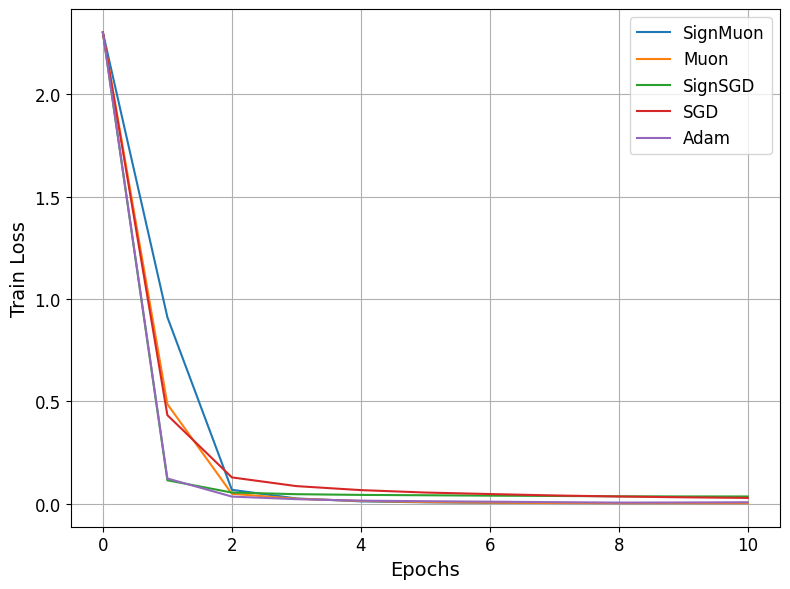
\includegraphics[width=\textwidth]{images/centralized_images/mnist_train_loss.png} 
%         \caption{Train Loss}
%     \end{subfigure}
%     \hfill
%     \begin{subfigure}[b]{0.48\textwidth}
%         \centering
%         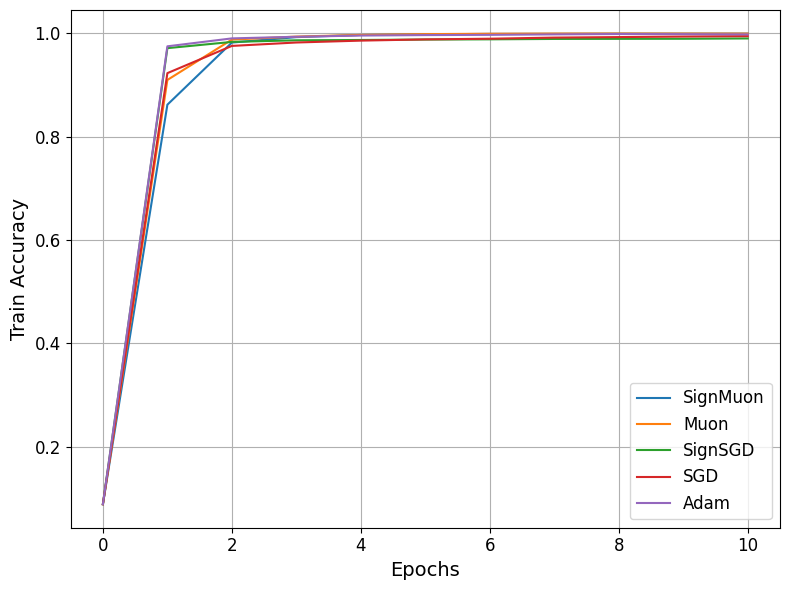
\includegraphics[width=\textwidth]{images/centralized_images/mnist_train_acc.png} 
%         \caption{Train Accuracy}
%     \end{subfigure}
%     \caption{Централизованное обучение. Сравнение сходимости и точности различных алгоритмов оптимизации на обучении классификатора MNIST на тренировочной выборке.}
%     \label{fig:mnist_results_train}
% \end{figure}

% \begin{figure}[H]
%     \begin{subfigure}[b]{0.48\textwidth}
%         \centering
%         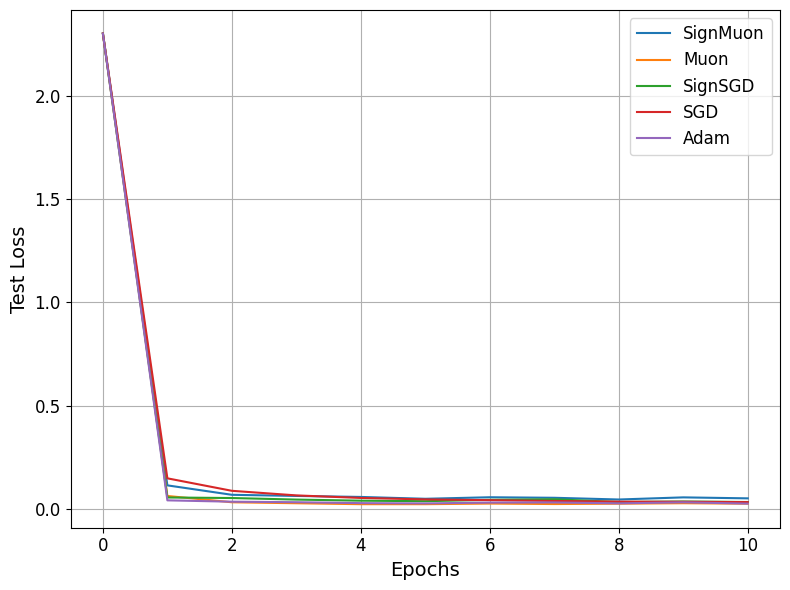
\includegraphics[width=\textwidth]{images/centralized_images/mnist_test_loss.png}
%         \caption{Test Loss}
%     \end{subfigure}
%     \hfill
%     \begin{subfigure}[b]{0.48\textwidth}
%         \centering
%         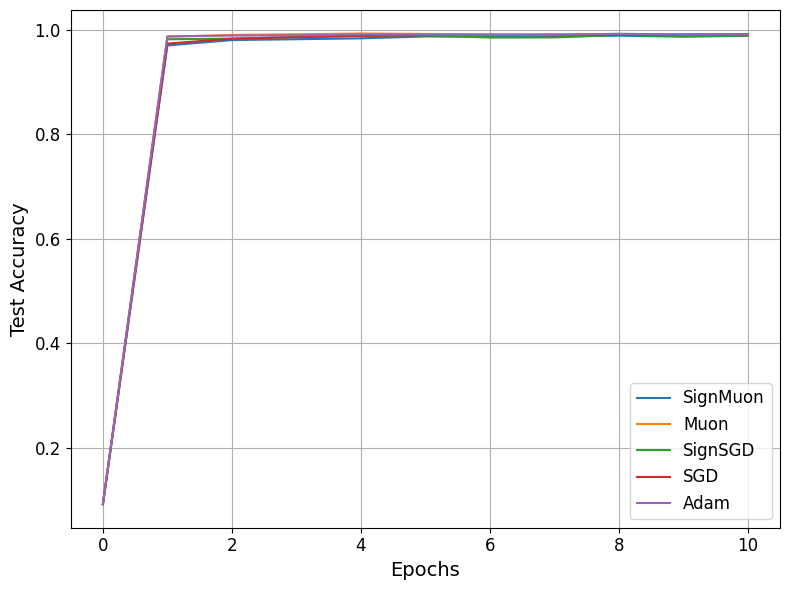
\includegraphics[width=\textwidth]{images/centralized_images/mnist_test_acc.png}
%         \caption{Test Accuracy}
%     \end{subfigure}
%     \caption{Централизованный сценарий. Сравнение сходимости и точности различных алгоритмов оптимизации на обучении классификатора MNIST на тестовой выборке.}
%     \label{fig:mnist_results}
% \end{figure}

\begin{figure}[H]
    \centering
    \begin{subfigure}[b]{0.48\textwidth}
        \centering
        
\includegraphics[width=\textwidth]{images/centralized_images/train_loss_resnet.png} 
        \caption{Train Loss}
    \end{subfigure}
    \hfill
    \begin{subfigure}[b]{0.48\textwidth}
        \centering
        
\includegraphics[width=\textwidth]{images/centralized_images/train_acc_resnet.png} 
        \caption{Train Accuracy}
    \end{subfigure}
    \caption{Централизованный сценарий. Сравнение сходимости и точности различных алгоритмов оптимизации на обучении классификатора CIFAR-10 на тренировочной выборке.}
    \label{fig:cifar_results_train}
\end{figure}

\begin{figure}[H]
    \begin{subfigure}[b]{0.48\textwidth}
        \centering
        
\includegraphics[width=\textwidth]{images/centralized_images/test_loss_resnet.png}
        \caption{Test Loss}
    \end{subfigure}
    \hfill
    \begin{subfigure}[b]{0.48\textwidth}
        \centering
        
\includegraphics[width=\textwidth]{images/centralized_images/test_acc_resnet.png}
        \caption{Test Accuracy}
    \end{subfigure}
    \caption{Централизованный сценарий. Сравнение сходимости и точности различных алгоритмов оптимизации на обучении классификатора CIFAR-10 на тестовой выборке.}
    \label{fig:cifar_results}
\end{figure}

\subsection{Результаты федеративного обучения. Эксперимент 1}\label{app:results_fed:1}

\begin{table}[H]
\centering
\caption{CIFAR10 -- Федеративное обучение. Эксперимент 1. Масштабируемость алгоритма SignMuon.}
\label{tab:exp_1}
\small
\renewcommand{\arraystretch}{1.2}
\begin{tabular}{|c|c|c|c|c|c|c|c|c|}
\hline
\textbf{Dataset} & \textbf{Optimizer} & \textbf{Rounds} & \textbf{Clients} & \textbf{Steps} & \textbf{Batch} & \textbf{LR} & \textbf{Mom} & \textbf{Test Acc} \\
\hline
\multirow{5}{*}{CIFAR-10} & \multirow{5}{*}{SignMuon} & \multirow{5}{*}{2000} & 1 & \multirow{5}{*}{1} & \multirow{5}{*}{64} & \multirow{5}{*}{0.001} & \multirow{5}{*}{0.9} & 76.13\% \\
\cline{4-4} \cline{9-9}
 & & & 3 & & & & & 81.24\% \\
\cline{4-4} \cline{9-9}
 & & & 5 & & & & & 82.87\% \\
\cline{4-4} \cline{4-4} \cline{9-9}
 & & & 7 & & & & & 83.54\% \\
\cline{4-4} \cline{9-9}
 & & & 9 & & & & & \textbf{84.03\%} \\
\hline
\end{tabular}
\end{table}

\begin{figure}[H]
    \centering
    \begin{subfigure}[b]{0.48\textwidth}
        \centering
        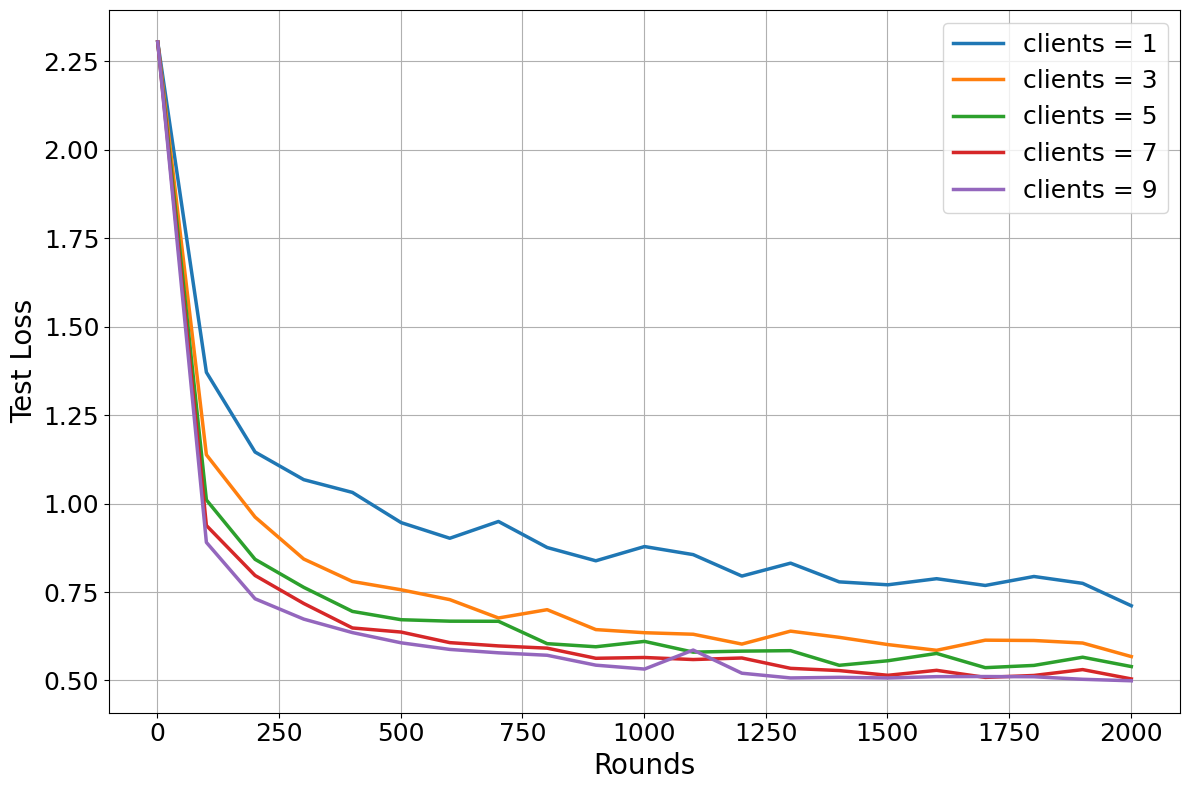
\includegraphics[width=\textwidth]{images/federated_images/signmuon_loss.png} 
        \caption{Test Loss}
    \end{subfigure}
    \hfill
    \begin{subfigure}[b]{0.48\textwidth}
        \centering
        
\includegraphics[width=\textwidth]{images/federated_images/signmuon_acc.png}
        \caption{Test Accuracy}
    \end{subfigure}
    \caption{Федеративное обучение. Эксперимент 1. Масштабируемость алгоритма SignMuon.}
    \label{fig:exp_1}
\end{figure}


\subsection{Результаты федеративного обучения. Эксперимент 2}\label{app:results_fed:2}
\begin{table}[H]
\centering
\caption{CIFAR10 -- Федеративное обучение. Эксперимент 2. Сравнение разных алгоритмов при числе узлов n=3.}
\label{tab:exp_2}
\small
\renewcommand{\arraystretch}{1.2}
\begin{tabular}{|c|c|c|c|c|c|c|c|c|}
\hline
\textbf{Dataset} & \textbf{Optimizer} & \textbf{Rounds} & \textbf{Clients} & \textbf{Steps} & \textbf{Batch} & \textbf{LR} & \textbf{Mom} & \textbf{Test Acc} \\
\hline
\multirow{6}{*}{CIFAR-10} & SignMuon & \multirow{6}{*}{2000} & \multirow{6}{*}{3} & \multirow{6}{*}{1} & \multirow{6}{*}{64} & 0.001 & \multirow{6}{*}{0.9} & 81.24\% \\
\cline{2-2} \cline{7-7} \cline{9-9}
 & Muon & & & & & 0.05 & & \textbf{81.27\%} \\
\cline{2-2} \cline{7-7} \cline{9-9}
 & SignSGD & & & & & 0.001 & & 65.96\% \\
\cline{2-2} \cline{7-7} \cline{9-9}
 & SGD & & & & & 0.03 & & 76.77\% \\
\cline{2-2} \cline{7-7} \cline{9-9}
 & Adam & & & & & 0.001 & & 70.83\% \\
\cline{2-2} \cline{7-7} \cline{9-9}
 & SignMuon\_EF & & & & & 0.02 & & 75.92\% \\
\hline
\end{tabular}
\end{table}

\begin{figure}[H]
    \centering
    \begin{subfigure}[b]{0.48\textwidth}
        \centering
        
\includegraphics[width=\textwidth]{images/federated_images/3_1_loss.png} 
        \caption{Test Loss}
    \end{subfigure}
    \hfill
    \begin{subfigure}[b]{0.48\textwidth}
        \centering
        
\includegraphics[width=\textwidth]{images/federated_images/3_1_acc.png}
        \caption{Test Accuracy}
    \end{subfigure}
    \caption{Федеративное обучение. Эксперимент 2. Сравнение разных алгоритмов при числе узлов n=3.}
    \label{fig:exp_2}
\end{figure}

\subsection{Результаты федеративного обучения. Эксперимент 3}\label{app:results_fed:3}
\begin{figure}[H]
    \centering
    \begin{subfigure}[b]{0.48\textwidth}
        \centering
        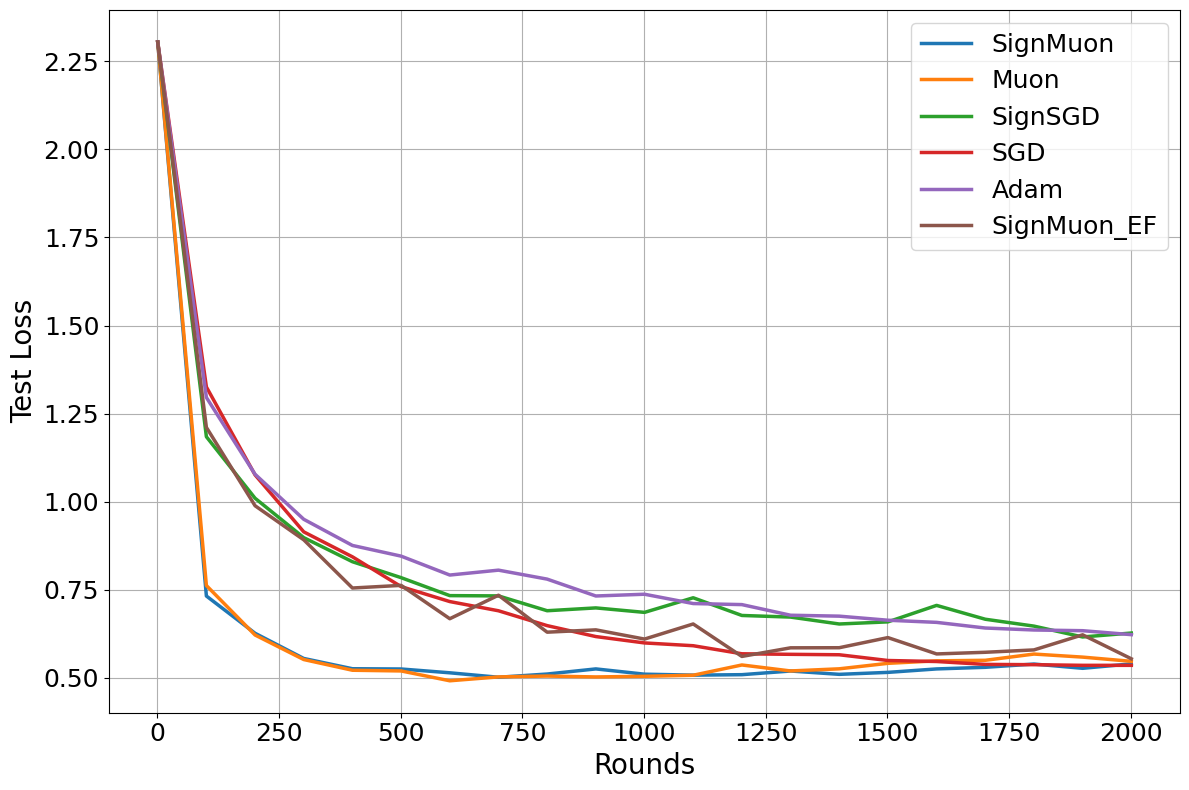
\includegraphics[width=\textwidth]{images/federated_images/10_3_loss.png} 
        \caption{Test Loss}
    \end{subfigure}
    \hfill
    \begin{subfigure}[b]{0.48\textwidth}
        \centering
        
\includegraphics[width=\textwidth]{images/federated_images/10_3_acc.png}
        \caption{Test Accuracy}
    \end{subfigure}
    \caption{Федеративное обучение. Эксперимент 3. Сравнение разных алгоритмов при числе узлов N=10.}
    \label{fig:exp_3}
\end{figure}


\end{document}